% Options for packages loaded elsewhere
\PassOptionsToPackage{unicode}{hyperref}
\PassOptionsToPackage{hyphens}{url}
\PassOptionsToPackage{dvipsnames,svgnames,x11names}{xcolor}
%
\documentclass[
  letterpaper,
  DIV=11,
  numbers=noendperiod]{scrartcl}

\usepackage{amsmath,amssymb}
\usepackage{iftex}
\ifPDFTeX
  \usepackage[T1]{fontenc}
  \usepackage[utf8]{inputenc}
  \usepackage{textcomp} % provide euro and other symbols
\else % if luatex or xetex
  \usepackage{unicode-math}
  \defaultfontfeatures{Scale=MatchLowercase}
  \defaultfontfeatures[\rmfamily]{Ligatures=TeX,Scale=1}
\fi
\usepackage{lmodern}
\ifPDFTeX\else  
    % xetex/luatex font selection
\fi
% Use upquote if available, for straight quotes in verbatim environments
\IfFileExists{upquote.sty}{\usepackage{upquote}}{}
\IfFileExists{microtype.sty}{% use microtype if available
  \usepackage[]{microtype}
  \UseMicrotypeSet[protrusion]{basicmath} % disable protrusion for tt fonts
}{}
\makeatletter
\@ifundefined{KOMAClassName}{% if non-KOMA class
  \IfFileExists{parskip.sty}{%
    \usepackage{parskip}
  }{% else
    \setlength{\parindent}{0pt}
    \setlength{\parskip}{6pt plus 2pt minus 1pt}}
}{% if KOMA class
  \KOMAoptions{parskip=half}}
\makeatother
\usepackage{xcolor}
\setlength{\emergencystretch}{3em} % prevent overfull lines
\setcounter{secnumdepth}{-\maxdimen} % remove section numbering
% Make \paragraph and \subparagraph free-standing
\ifx\paragraph\undefined\else
  \let\oldparagraph\paragraph
  \renewcommand{\paragraph}[1]{\oldparagraph{#1}\mbox{}}
\fi
\ifx\subparagraph\undefined\else
  \let\oldsubparagraph\subparagraph
  \renewcommand{\subparagraph}[1]{\oldsubparagraph{#1}\mbox{}}
\fi


\providecommand{\tightlist}{%
  \setlength{\itemsep}{0pt}\setlength{\parskip}{0pt}}\usepackage{longtable,booktabs,array}
\usepackage{calc} % for calculating minipage widths
% Correct order of tables after \paragraph or \subparagraph
\usepackage{etoolbox}
\makeatletter
\patchcmd\longtable{\par}{\if@noskipsec\mbox{}\fi\par}{}{}
\makeatother
% Allow footnotes in longtable head/foot
\IfFileExists{footnotehyper.sty}{\usepackage{footnotehyper}}{\usepackage{footnote}}
\makesavenoteenv{longtable}
\usepackage{graphicx}
\makeatletter
\def\maxwidth{\ifdim\Gin@nat@width>\linewidth\linewidth\else\Gin@nat@width\fi}
\def\maxheight{\ifdim\Gin@nat@height>\textheight\textheight\else\Gin@nat@height\fi}
\makeatother
% Scale images if necessary, so that they will not overflow the page
% margins by default, and it is still possible to overwrite the defaults
% using explicit options in \includegraphics[width, height, ...]{}
\setkeys{Gin}{width=\maxwidth,height=\maxheight,keepaspectratio}
% Set default figure placement to htbp
\makeatletter
\def\fps@figure{htbp}
\makeatother
\newlength{\cslhangindent}
\setlength{\cslhangindent}{1.5em}
\newlength{\csllabelwidth}
\setlength{\csllabelwidth}{3em}
\newlength{\cslentryspacingunit} % times entry-spacing
\setlength{\cslentryspacingunit}{\parskip}
\newenvironment{CSLReferences}[2] % #1 hanging-ident, #2 entry spacing
 {% don't indent paragraphs
  \setlength{\parindent}{0pt}
  % turn on hanging indent if param 1 is 1
  \ifodd #1
  \let\oldpar\par
  \def\par{\hangindent=\cslhangindent\oldpar}
  \fi
  % set entry spacing
  \setlength{\parskip}{#2\cslentryspacingunit}
 }%
 {}
\usepackage{calc}
\newcommand{\CSLBlock}[1]{#1\hfill\break}
\newcommand{\CSLLeftMargin}[1]{\parbox[t]{\csllabelwidth}{#1}}
\newcommand{\CSLRightInline}[1]{\parbox[t]{\linewidth - \csllabelwidth}{#1}\break}
\newcommand{\CSLIndent}[1]{\hspace{\cslhangindent}#1}

\KOMAoption{captions}{tableheading}
\makeatletter
\@ifpackageloaded{tcolorbox}{}{\usepackage[skins,breakable]{tcolorbox}}
\@ifpackageloaded{fontawesome5}{}{\usepackage{fontawesome5}}
\definecolor{quarto-callout-color}{HTML}{909090}
\definecolor{quarto-callout-note-color}{HTML}{0758E5}
\definecolor{quarto-callout-important-color}{HTML}{CC1914}
\definecolor{quarto-callout-warning-color}{HTML}{EB9113}
\definecolor{quarto-callout-tip-color}{HTML}{00A047}
\definecolor{quarto-callout-caution-color}{HTML}{FC5300}
\definecolor{quarto-callout-color-frame}{HTML}{acacac}
\definecolor{quarto-callout-note-color-frame}{HTML}{4582ec}
\definecolor{quarto-callout-important-color-frame}{HTML}{d9534f}
\definecolor{quarto-callout-warning-color-frame}{HTML}{f0ad4e}
\definecolor{quarto-callout-tip-color-frame}{HTML}{02b875}
\definecolor{quarto-callout-caution-color-frame}{HTML}{fd7e14}
\makeatother
\makeatletter
\makeatother
\makeatletter
\makeatother
\makeatletter
\@ifpackageloaded{caption}{}{\usepackage{caption}}
\AtBeginDocument{%
\ifdefined\contentsname
  \renewcommand*\contentsname{Table of contents}
\else
  \newcommand\contentsname{Table of contents}
\fi
\ifdefined\listfigurename
  \renewcommand*\listfigurename{List of Figures}
\else
  \newcommand\listfigurename{List of Figures}
\fi
\ifdefined\listtablename
  \renewcommand*\listtablename{List of Tables}
\else
  \newcommand\listtablename{List of Tables}
\fi
\ifdefined\figurename
  \renewcommand*\figurename{Figure}
\else
  \newcommand\figurename{Figure}
\fi
\ifdefined\tablename
  \renewcommand*\tablename{Table}
\else
  \newcommand\tablename{Table}
\fi
}
\@ifpackageloaded{float}{}{\usepackage{float}}
\floatstyle{ruled}
\@ifundefined{c@chapter}{\newfloat{codelisting}{h}{lop}}{\newfloat{codelisting}{h}{lop}[chapter]}
\floatname{codelisting}{Listing}
\newcommand*\listoflistings{\listof{codelisting}{List of Listings}}
\makeatother
\makeatletter
\@ifpackageloaded{caption}{}{\usepackage{caption}}
\@ifpackageloaded{subcaption}{}{\usepackage{subcaption}}
\makeatother
\makeatletter
\@ifpackageloaded{tcolorbox}{}{\usepackage[skins,breakable]{tcolorbox}}
\makeatother
\makeatletter
\@ifundefined{shadecolor}{\definecolor{shadecolor}{rgb}{.97, .97, .97}}
\makeatother
\makeatletter
\makeatother
\makeatletter
\makeatother
\ifLuaTeX
  \usepackage{selnolig}  % disable illegal ligatures
\fi
\IfFileExists{bookmark.sty}{\usepackage{bookmark}}{\usepackage{hyperref}}
\IfFileExists{xurl.sty}{\usepackage{xurl}}{} % add URL line breaks if available
\urlstyle{same} % disable monospaced font for URLs
\hypersetup{
  pdftitle={Defining and Assessing Learning},
  pdfauthor={Ovande Furtado Jr},
  colorlinks=true,
  linkcolor={blue},
  filecolor={Maroon},
  citecolor={Blue},
  urlcolor={Blue},
  pdfcreator={LaTeX via pandoc}}

\title{Defining and Assessing Learning}
\usepackage{etoolbox}
\makeatletter
\providecommand{\subtitle}[1]{% add subtitle to \maketitle
  \apptocmd{\@title}{\par {\large #1 \par}}{}{}
}
\makeatother
\subtitle{KIN 377 - Motor Learning}
\author{Ovande Furtado Jr}
\date{2023-09-11}

\begin{document}
\maketitle
\ifdefined\Shaded\renewenvironment{Shaded}{\begin{tcolorbox}[frame hidden, breakable, interior hidden, enhanced, boxrule=0pt, sharp corners, borderline west={3pt}{0pt}{shadecolor}]}{\end{tcolorbox}}\fi

\hypertarget{overview}{%
\subsection{Overview}\label{overview}}

People who assess learning must make inferences from observing
performance during practice and tests\hspace{0pt} Magill \& Anderson
(2020).

\hypertarget{pop-up-quiz}{%
\subsection{Pop-up Quiz}\label{pop-up-quiz}}

\hypertarget{learning-objectives}{%
\subsection{Learning Objectives}\label{learning-objectives}}

\begin{itemize}
\tightlist
\item
  Define and distinguish between the terms performance and
  learning\hspace{0pt}
\item
  Identify six general performance characteristics typically observable
  as motor skill learning occurs\hspace{0pt}
\item
  Describe several different methods to assess motor skill
  learning\hspace{0pt}
\item
  Discuss two reasons performance during the practice of a motor skill
  may misrepresent the amount of learning that occurred during
  practice\hspace{0pt}
\end{itemize}

\hypertarget{how-would-you-tell}{%
\subsection{How would you tell?}\label{how-would-you-tell}}

\begin{enumerate}
\def\labelenumi{\arabic{enumi}.}
\item
  How do you determine whether performers are learning what you are
  teaching them?\hspace{0pt}
\item
  How can progress be evaluated?

  Watch the video depicted in the link below:

  \url{https://youtu.be/HCe0cs-qVF8\hspace{0pt}}
\end{enumerate}

\begin{tcolorbox}[enhanced jigsaw, opacitybacktitle=0.6, coltitle=black, colbacktitle=quarto-callout-tip-color!10!white, bottomtitle=1mm, arc=.35mm, colframe=quarto-callout-tip-color-frame, left=2mm, bottomrule=.15mm, toprule=.15mm, toptitle=1mm, breakable, opacityback=0, titlerule=0mm, title=\textcolor{quarto-callout-tip-color}{\faLightbulb}\hspace{0.5em}{Concerning the video above}, rightrule=.15mm, leftrule=.75mm, colback=white]

\begin{enumerate}
\def\labelenumi{\arabic{enumi}.}
\tightlist
\item
  Do you think the performer has learned the backhand and forwhand
  skills?
\item
  How can you be certain that what you are observing is the result of
  \texttt{learning} and not just luck?\hspace{0pt}
\end{enumerate}

\end{tcolorbox}

It is not possible to infer about learning by simply observing this
performance.

\hypertarget{performance-vs-learning}{%
\subsection{Performance vs Learning}\label{performance-vs-learning}}

\begin{tcolorbox}[enhanced jigsaw, opacitybacktitle=0.6, coltitle=black, colbacktitle=quarto-callout-note-color!10!white, bottomtitle=1mm, arc=.35mm, colframe=quarto-callout-note-color-frame, left=2mm, bottomrule=.15mm, toprule=.15mm, toptitle=1mm, breakable, opacityback=0, titlerule=0mm, title=\textcolor{quarto-callout-note-color}{\faInfo}\hspace{0.5em}{Note}, rightrule=.15mm, leftrule=.75mm, colback=white]

Learning: A change in the capability to perform a skill that must be
inferred from a relatively permanent improvement in performance as a
result of practice or experience (Magill \& Anderson, 2020)

\end{tcolorbox}

\begin{itemize}
\tightlist
\item
  Performance

  \begin{itemize}
  \tightlist
  \item
    Execution of a skill at a specific time and in a specific
    location\hspace{0pt}
  \item
    This is the observable behavior\hspace{0pt}
  \end{itemize}
\item
  Learning\hspace{0pt}

  \begin{itemize}
  \tightlist
  \item
    Not directly observable\hspace{0pt}
  \item
    Must be inferred from observable behavior\hspace{0pt}
  \end{itemize}
\end{itemize}

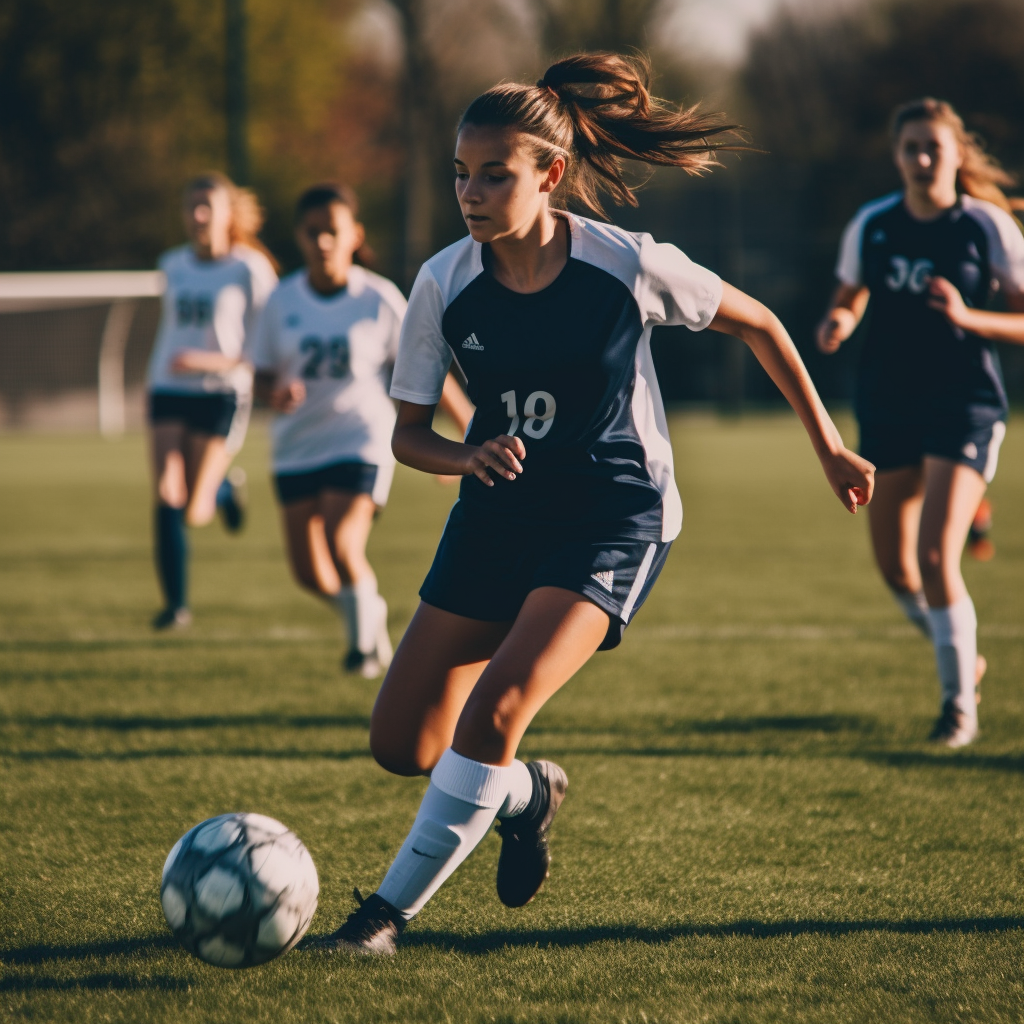
\includegraphics[width=4.6875in,height=\textheight]{ma-ch11_files/mediabag/drfurtado_a_girl_hea.png}

\hypertarget{performance-vs-learning-cont}{%
\subsection{Performance vs Learning,
cont}\label{performance-vs-learning-cont}}

\textbf{Performance}

\begin{itemize}
\tightlist
\item
  Observable behavior
\item
  Temporary
\item
  May not be due to practice
\item
  May be influenced by performance variables
\end{itemize}

\textbf{Learning}

\begin{itemize}
\tightlist
\item
  Inferred from performance characteristics (discussed later)
\item
  Relatively permanent
\item
  Due to practice
\item
  Not influenced by performance variables

  \begin{itemize}
  \tightlist
  \item
    e.g., fatigue may influence performance, but not impact learning
  \end{itemize}
\end{itemize}

\hypertarget{performance-vs-learning-cont-1}{%
\subsection{Performance vs Learning,
cont}\label{performance-vs-learning-cont-1}}

From the definition:

\ldots the person has increased his/her capability, or potential, to
perform a skill.

Whether or not the person performs the skill in a way that is consistent
with this potential will depend on the presence of what are known as
\texttt{PERFORMANCE\ VARIABLES}.

\begin{quote}
Performance variables such as alertness, anxiety, fatigue, etc. can
influence an individual's performance but not reflect their learning.
These factors can distort the representation of learning and must be
considered when evaluating learning to ensure accurate deductions are
made. (Magill \& Anderson, 2020, p. 263).
\end{quote}

\hypertarget{performance-characteristics-of-skill-learning}{%
\subsection{Performance characteristics of skill
learning}\label{performance-characteristics-of-skill-learning}}

\texttt{Improvement}

\begin{itemize}
\tightlist
\item
  Over a period of time, there has been improvement in the performance
  of the skill.
\item
  This means that the person performs at a higher level of skill at some
  later time, then at some previous time.
\item
  Performance may get worse as practice continues due to bad habits.
\item
  Plateaus and regressions in performance are often seen during skill
  acquisition.
\item
  Still improvements are apparent when learning is viewed over a longer
  time scale.
\end{itemize}

\hypertarget{performance-characteristics-of-skill-learning-1}{%
\subsection{Performance characteristics of skill
learning}\label{performance-characteristics-of-skill-learning-1}}

\texttt{Consistency}

\begin{itemize}
\tightlist
\item
  As learning progresses, performance becomes increasingly more
  consistent.
\item
  The performance is similar from one attempt to another
\item
  Consistency is typically quite variable from one attempt to another
  early in learning
\item
  It becomes more consistent as learning takes place
\end{itemize}

\hypertarget{performance-characteristics-of-skill-learning-2}{%
\subsection{Performance characteristics of skill
learning}\label{performance-characteristics-of-skill-learning-2}}

\texttt{Stability}

\begin{itemize}
\tightlist
\item
  as learning progresses, performance stability increases
\item
  stability refers to the influence on skill performance of
  perturbations, which are internal or external conditions that can
  disrupt performance
\item
  stress is an example of internal perturbation
\item
  the weather or an issue with the person's shoes are examples of
  external perturbations.
\item
  there are limits to the amount of perturbation that can be overcome
\end{itemize}

\hypertarget{performance-characteristics-of-skill-learning-3}{%
\subsection{Performance characteristics of skill
learning}\label{performance-characteristics-of-skill-learning-3}}

\texttt{Persistence}

\begin{itemize}
\tightlist
\item
  The improved performance capability is marked by an increasing amount
  of persistence
\item
  As the person progresses in learning the skill, the improved
  performance capability lasts over increasing periods of time
\end{itemize}

\hypertarget{performance-characteristics-of-skill-learning-4}{%
\subsection{Performance characteristics of skill
learning}\label{performance-characteristics-of-skill-learning-4}}

\texttt{Adaptability}

\begin{itemize}
\tightlist
\item
  the improved performance is adaptable to a variety of performance
  context characteristics
\item
  something is different every time we perform a skill
\item
  successful skill performance requires adaptability to changes in
  personal, task, and or environmental characteristics
\end{itemize}

\begin{tcolorbox}[enhanced jigsaw, opacitybacktitle=0.6, coltitle=black, colbacktitle=quarto-callout-note-color!10!white, bottomtitle=1mm, arc=.35mm, colframe=quarto-callout-note-color-frame, left=2mm, bottomrule=.15mm, toprule=.15mm, toptitle=1mm, breakable, opacityback=0, titlerule=0mm, title=\textcolor{quarto-callout-note-color}{\faInfo}\hspace{0.5em}{Note}, rightrule=.15mm, leftrule=.75mm, colback=white]

Stability and adaptability are both important, but for different
reasons. Stability provides a reliable foundation for performance, while
adaptability allows for flexibility and innovation.

\end{tcolorbox}

\hypertarget{performance-characteristics-of-skill-learning-5}{%
\subsection{Performance characteristics of skill
learning}\label{performance-characteristics-of-skill-learning-5}}

\texttt{Reduction\ in\ attention\ demands}

\begin{itemize}
\tightlist
\item
  Reduction in the amount of attention demanded to perform the skill
\item
  As learning progresses, the learner can more easily perform another
  activity simultaneously
\end{itemize}

\hypertarget{learning-assessment-techniques}{%
\subsection{Learning Assessment
Techniques}\label{learning-assessment-techniques}}

\texttt{Performance\ curves\ for\ outcome\ measures}

\begin{itemize}
\tightlist
\item
  provide a way to observe performance \texttt{improvement} and
  \texttt{consistency} over a period of time\hspace{0pt}
\end{itemize}

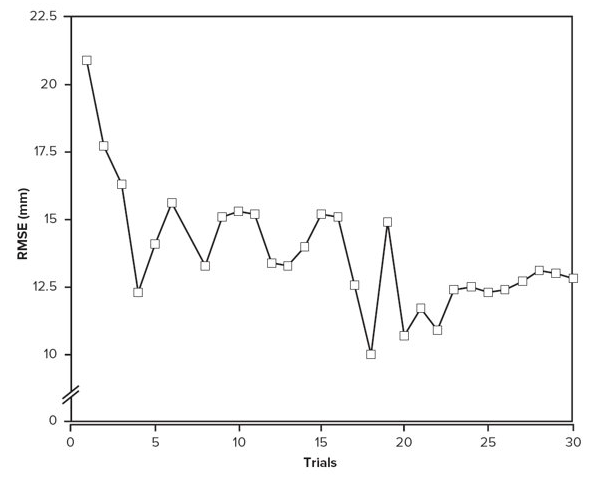
\includegraphics{images/Screenshot 2023-09-11 at 11.09.48 AM.png}

\hypertarget{type-of-performance-curves}{%
\subsection{Type of Performance
Curves}\label{type-of-performance-curves}}

\begin{itemize}
\tightlist
\item
  Linear

  \begin{itemize}
  \tightlist
  \item
    Proportional performance increases over time.\hspace{0pt}
  \end{itemize}
\item
  Negatively accelerated.\hspace{0pt}

  \begin{itemize}
  \tightlist
  \item
    Large amount of improvement occurs early but slows
    later.\hspace{0pt}
  \end{itemize}
\item
  Positively accelerated

  \begin{itemize}
  \tightlist
  \item
    Slight performance gain early in practice, but substantial
    improvement later.\hspace{0pt}
  \end{itemize}
\item
  Ogive or S-shaped\hspace{0pt}

  \begin{itemize}
  \tightlist
  \item
    Combination of A, B, and C curves.\hspace{0pt}
  \end{itemize}
\end{itemize}

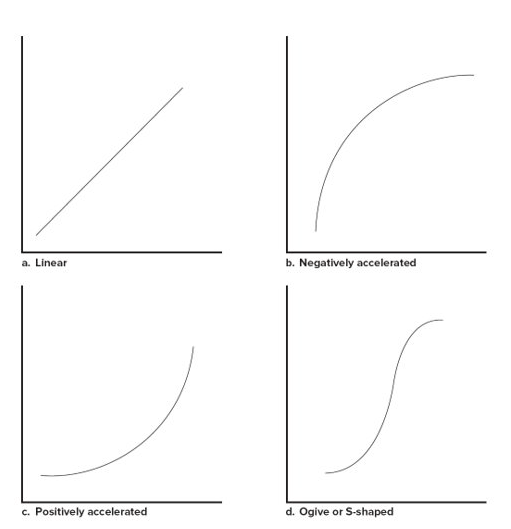
\includegraphics{images/Screenshot 2023-09-11 at 11.13.16 AM.png}

\hypertarget{learning-assessment-techniques-1}{%
\subsection{Learning Assessment
Techniques}\label{learning-assessment-techniques-1}}

\texttt{Performance\ curves\ for\ kinematic\ measures}

\begin{itemize}
\tightlist
\item
  Kinematic: study of the motion itself, without considering the forces
\item
  Improvement: compare block trials 1-10 with 751-760
\item
  Consistency: compare the SD~block trials 1-10 with~751-760.
\end{itemize}

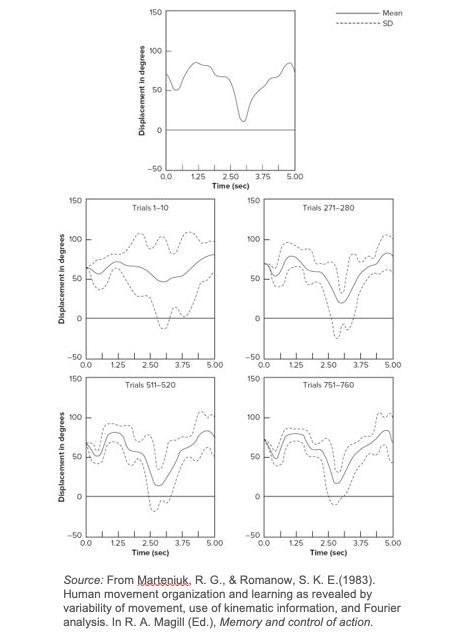
\includegraphics{images/Screenshot 2023-09-11 at 11.23.50 AM.png}

\hypertarget{learning-assessment-techniques-2}{%
\subsection{Learning Assessment
Techniques}\label{learning-assessment-techniques-2}}

\texttt{Retention\ tests}

\begin{itemize}
\tightlist
\item
  Assess \texttt{persistence} of an improved performance capability by
  requiring the performance of the practiced skill after a period of
  time during which the skill was not practiced
\item
  \textbf{Length of time} between the end of practice and the test is
  arbitrary
\end{itemize}

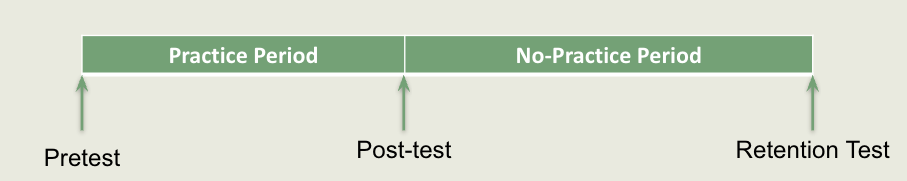
\includegraphics{images/Screenshot 2023-09-11 at 12.22.36 PM.png}

\hypertarget{learning-assessment-techniques-3}{%
\subsection{Learning Assessment
Techniques}\label{learning-assessment-techniques-3}}

\texttt{Transfer\ tests}

\begin{itemize}
\tightlist
\item
  Assess the acquired capability to \texttt{adapt} to performance
  situations and contexts that were not experienced during practice
\item
  Test usually involves performing the practiced skill \textbf{in a
  novel situation or context.}\hspace{0pt}

  \begin{itemize}
  \tightlist
  \item
    Availability of augmented feedback
  \item
    Physical environment
  \item
    Personal characteristics of the test taker
  \end{itemize}
\item
  Performing a skill that is a \textbf{novel variation} of the practiced
  skill.\hspace{0pt}

  \begin{itemize}
  \tightlist
  \item
    An aspect of adaptability.
  \end{itemize}
\end{itemize}

\hypertarget{learning-assessment-techniques-4}{%
\subsection{Learning Assessment
Techniques}\label{learning-assessment-techniques-4}}

\texttt{Coordination\ dynamics}

\begin{itemize}
\tightlist
\item
  graphical representations of movement coordination patterns during
  practice and tests provide a means of assessing the
  \texttt{consistency} and \texttt{stability} of coordination
  characteristics associated with performing a motor skill\hspace{0pt}
\end{itemize}

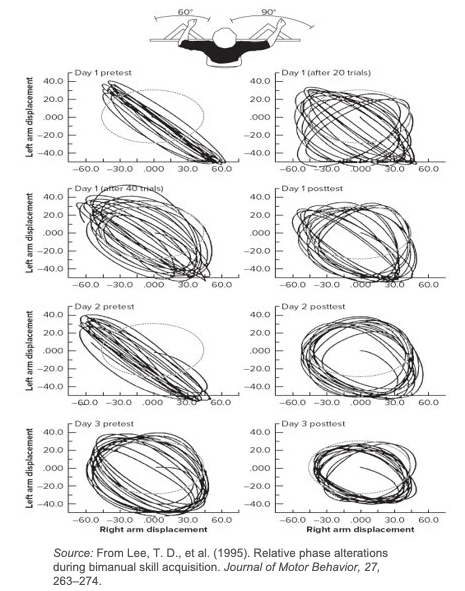
\includegraphics{images/Screenshot 2023-09-11 at 11.20.22 AM.png}

\hypertarget{learning-assessment-techniques-5}{%
\subsection{Learning Assessment
Techniques}\label{learning-assessment-techniques-5}}

\texttt{Dual-task\ procedure}

\begin{itemize}
\tightlist
\item
  Means of determining if \textbf{changes in attention demands} for a
  skill change as a learner \textbf{becomes more skillful}
\item
  Assesses the \texttt{attention\ \ demands} associated with perform­ing
  a skill
\item
  Attention demands are expected to decrease as amount of learning
  increases\hspace{0pt}
\item
  According to Kahneman's theory, this \textbf{change is predicted as a
  characteristic of learning}\hspace{0pt}

  \begin{itemize}
  \tightlist
  \item
    The procedure involves \textbf{assessing the effect on a primary
    task} when it is performed \textbf{concurrently with a secondary
    task}
  \end{itemize}
\end{itemize}

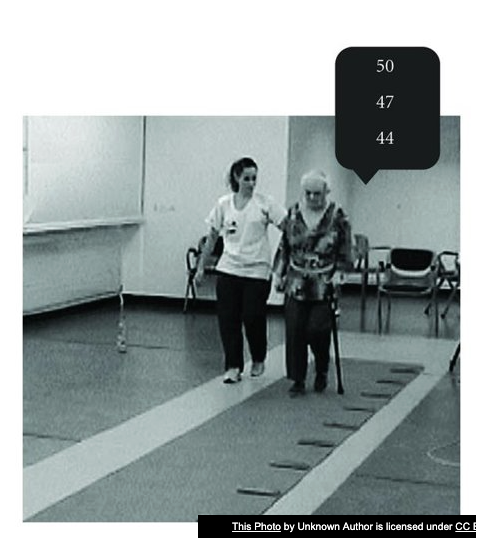
\includegraphics{images/Screenshot 2023-09-11 at 11.40.45 AM.png}

\hypertarget{practice-performance-may-misrepresent-learning}{%
\subsection{\texorpdfstring{\textbf{Practice Performance May
Misrepresent
Learning}\hspace{0pt}}{Practice Performance May Misrepresent Learning\hspace{0pt}}}\label{practice-performance-may-misrepresent-learning}}

Two reasons:\hspace{0pt}

\begin{itemize}
\tightlist
\item
  \textbf{Practice} may involve a performance variable that artificially
  \textbf{inflates} or \textbf{depresses performance}\hspace{0pt}
\item
  Practice may involve \textbf{performance plateaus}
\end{itemize}

\hypertarget{reason-1}{%
\subsection{Reason 1}\label{reason-1}}

\begin{itemize}
\tightlist
\item
  Certain~ performance variables can artificially inflate~ or~ depress~
  practice~ performance~ so~ that the observed performance during
  practice over­ or underestimates~ the~ amount~ a~ person~ has~ learned~
  during~ practice.
\end{itemize}

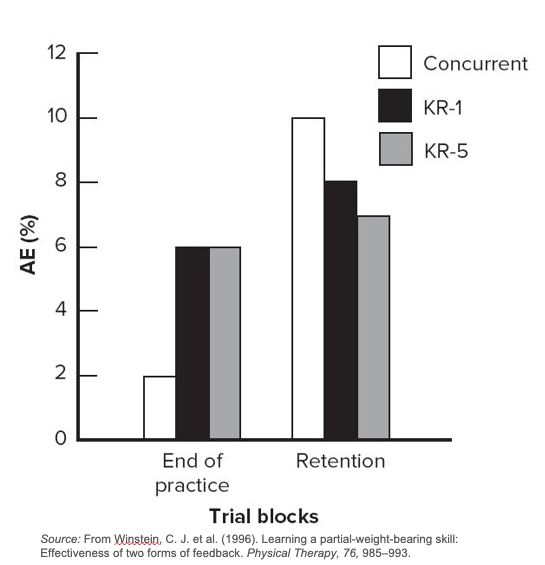
\includegraphics{images/Screenshot 2023-09-11 at 11.18.17 AM.png}

\hypertarget{reason-2}{%
\subsection{Reason 2}\label{reason-2}}

\begin{itemize}
\tightlist
\item
  Periods of time during which performance does not improve give the
  appearance that learning has stopped even though it has not.
\item
  Providing additional practice trials can establish a means of
  deter­mining~ whether learning continued during a performance plateau''
\end{itemize}

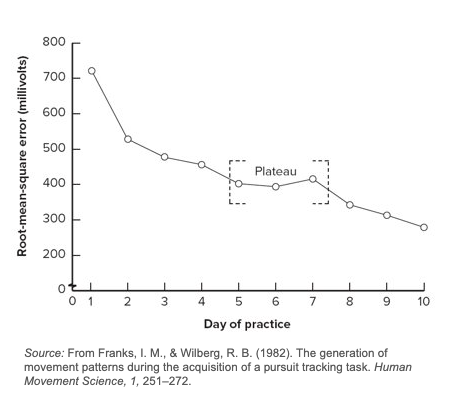
\includegraphics{images/Screenshot 2023-09-11 at 11.47.44 AM-01.png}

\hypertarget{section}{%
\subsection{\hspace{0pt}}\label{section}}

\hypertarget{references}{%
\subsection*{References}\label{references}}
\addcontentsline{toc}{subsection}{References}

\hypertarget{refs}{}
\begin{CSLReferences}{1}{0}
\leavevmode\vadjust pre{\hypertarget{ref-magill2020}{}}%
Magill, R. A., \& Anderson, D. (2020). \emph{Motor learning and control:
concepts and applications}. McGraw-Hill Education.
\url{https://www.bkstr.com/csunorthridgestore/product/motor-learning-and-control--concepts-and-applications-147614-1}

\end{CSLReferences}



\end{document}
